\begin{frame}
  \frametitle{Motivation/Goals}
  	\textbf{Motivation}
        \begin{itemize}
                \item Safeguard by design
                \item Model diversion inside facilities
                \item transition from LWR to SFR
        \end{itemize}
    \textbf{Goals}
    	\begin{itemize}
    		\item Detect diversion using signatures and observables.
    		\item Optimum detector and inspection locations in pyroprocessing
    		\item Characterize detection sensitivities and false positive rates
    	\end{itemize}
\end{frame}

\begin{frame}
	\frametitle{PyRe Archetype}
	\begin{columns}
		\column[t]{5cm}
		\begin{itemize}
			\item Facility containing multiple sub-processes:
			\begin{itemize}
				\item Separately handled.
				\item Independent transactions, possibility of diversion.
			\end{itemize}
			\item Operation setting impact efficiency.
			\item Generic facility:
			\begin{itemize}
				\item Multiple types of pyro plants.
				\item LWR vs SFR.
			\end{itemize}
		\end{itemize}
		\column[t]{6cm}
		\begin{figure}
			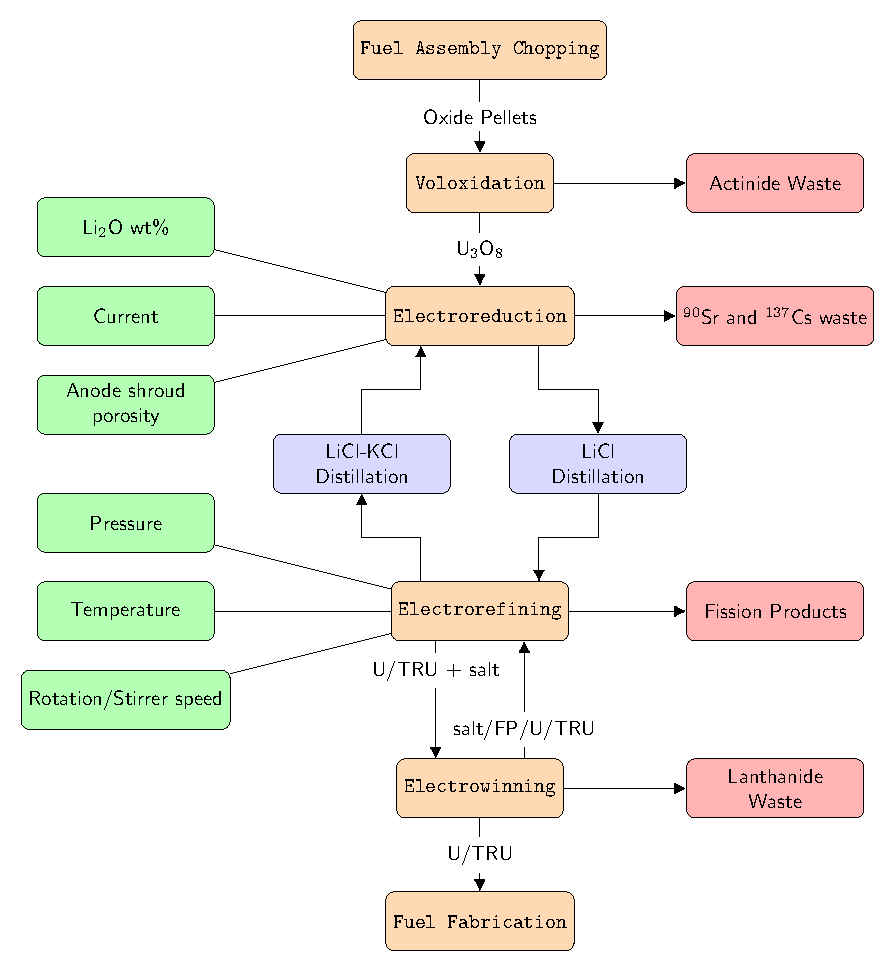
\includegraphics[width=\linewidth]{./images/westphal-pyre.pdf}
			\caption{PyRe flow diagram for LWR waste configuration.}
			\label{fig:pyre}
		\end{figure}
	\end{columns}
\end{frame}

\begin{frame}
\frametitle{Pyre - Diversion Options}
Material diversion occurs in two different modes: \textbf{nefarious} or \textbf{operator}.
\begin{itemize}
	\item \textbf{Nefarious Diversion} imagines diversion by a single bad actor with facility access.
	\item \textbf{Operator Diversion} imagines undeclared production.
\end{itemize}
\begin{figure}
	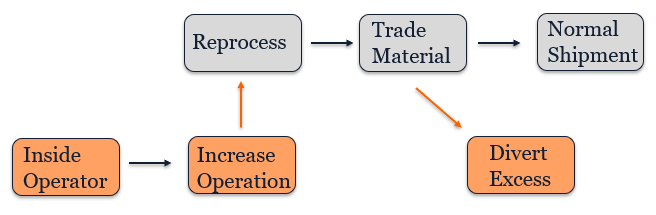
\includegraphics[width=0.7\linewidth]{./images/westphal-diversion}
	\caption{Operator vs nefarious diversion.}
	\label{fig:diversion}
\end{figure}
\end{frame}

\begin{frame}
	\frametitle{Diverter Class}
	\begin{columns}
		\column[t]{5cm}
		Inputs:
		\begin{itemize}
			\item Location
			\begin{itemize}
				\item Sub-process
				\item Operation Setting
			\end{itemize}
			\item Quantity
			\item Frequency
			\item Number of Diversions
		\end{itemize}
		\begin{block}{Purpose}
			The goal of a separate diverter class is to allow this method to be used by facilities other
			than pyre through a toolkit.
		\end{block}
		\column[t]{6cm}
		\begin{figure}
			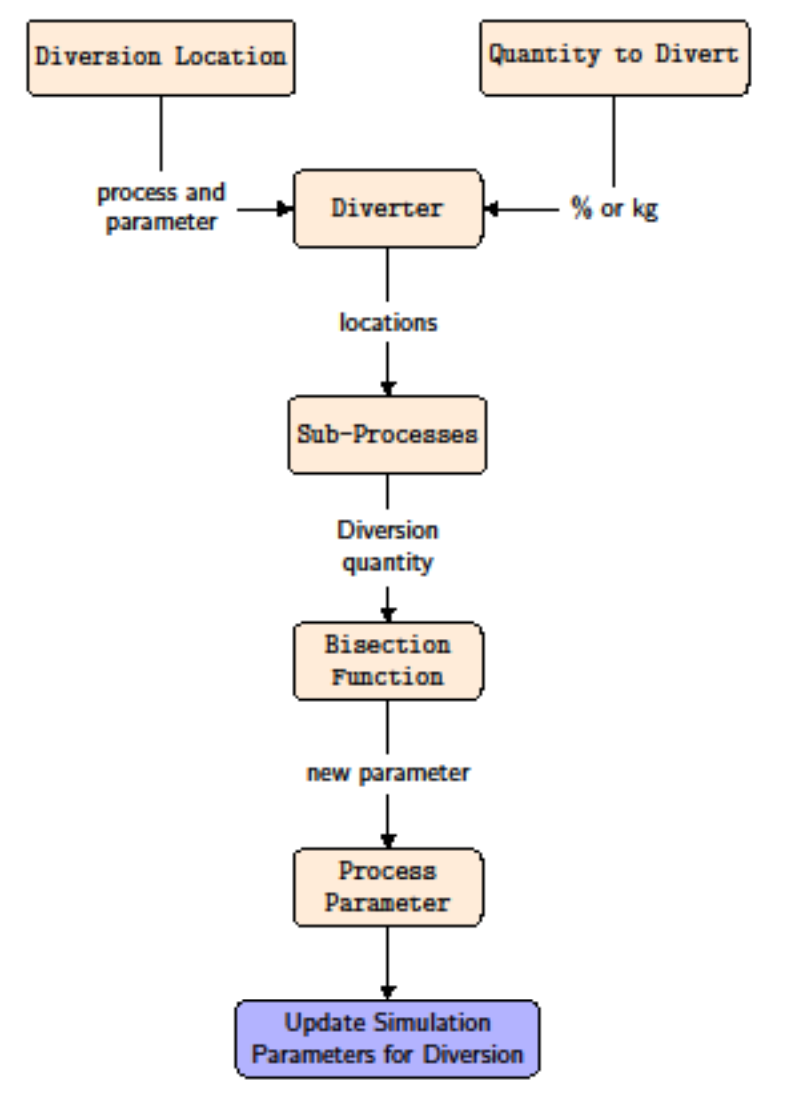
\includegraphics[width=0.8\linewidth]{images/diverter}
			\label{fig:diverter}
		\end{figure}
	\end{columns}
\end{frame}

\begin{frame}
\frametitle{Diversion Detection}
\begin{columns}
	\column[t]{5cm}
	\begin{block}{Diversion Detection}
		Material transactions are no longer a reliable method. Instead we use
		signatures and observables:
		\begin{itemize}
			\item Temperature, power draw, etc.
		\end{itemize}
		A Cumulative Sum change algorithm is used to detect any significant changes.
	\end{block}
	\column[t]{6cm}
	\begin{figure}
		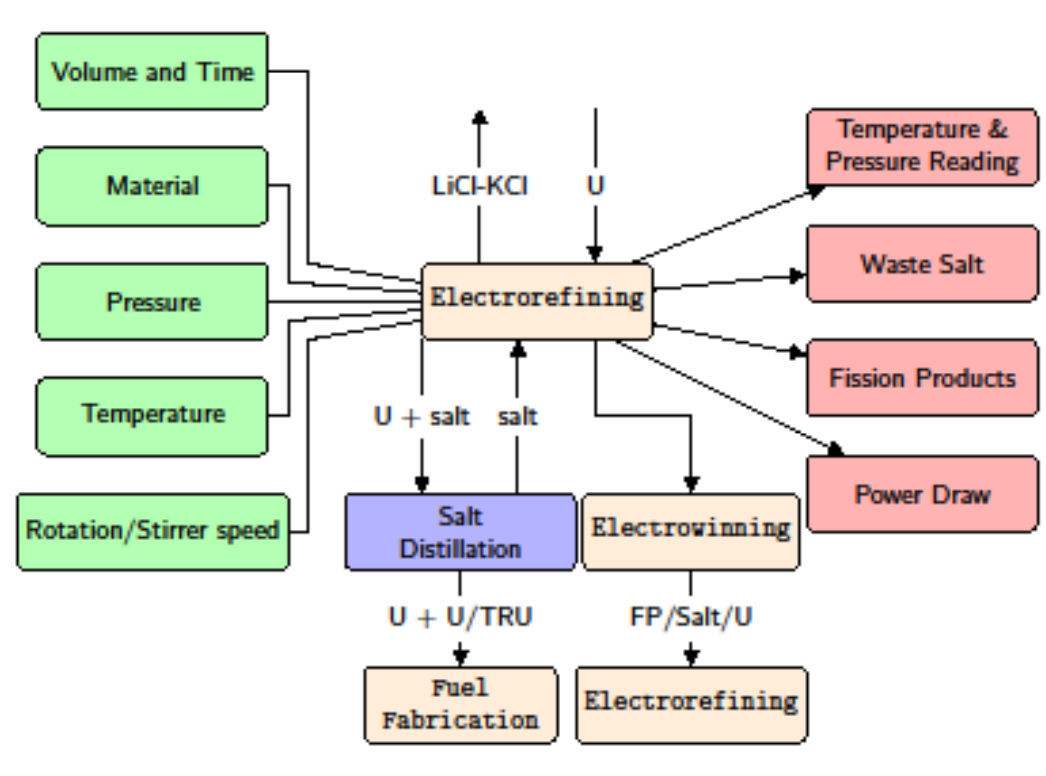
\includegraphics[width=\linewidth]{images/refining}
	\end{figure}
\end{columns}
\end{frame}

\begin{frame}
\frametitle{Transition Scenario}
A main attraction of pyroprocessing is the ability to handle LWR and
SFR waste.
\begin{itemize}
	\item To verify this capability in PyRe, we ran an EG01 – EG24 transition
	scenario.
	\item We want to observe the following:
	\begin{itemize}
		\item Appropriate deploying of PyRe
		\item Ability to meet demand of new SFRs
		\item Diversion capabilities
		\item Accurate transition from UOX to SFR fuels
	\end{itemize}
\end{itemize}
\end{frame}

\begin{frame}
\frametitle{Transition Scenario - Results}
\begin{figure}
	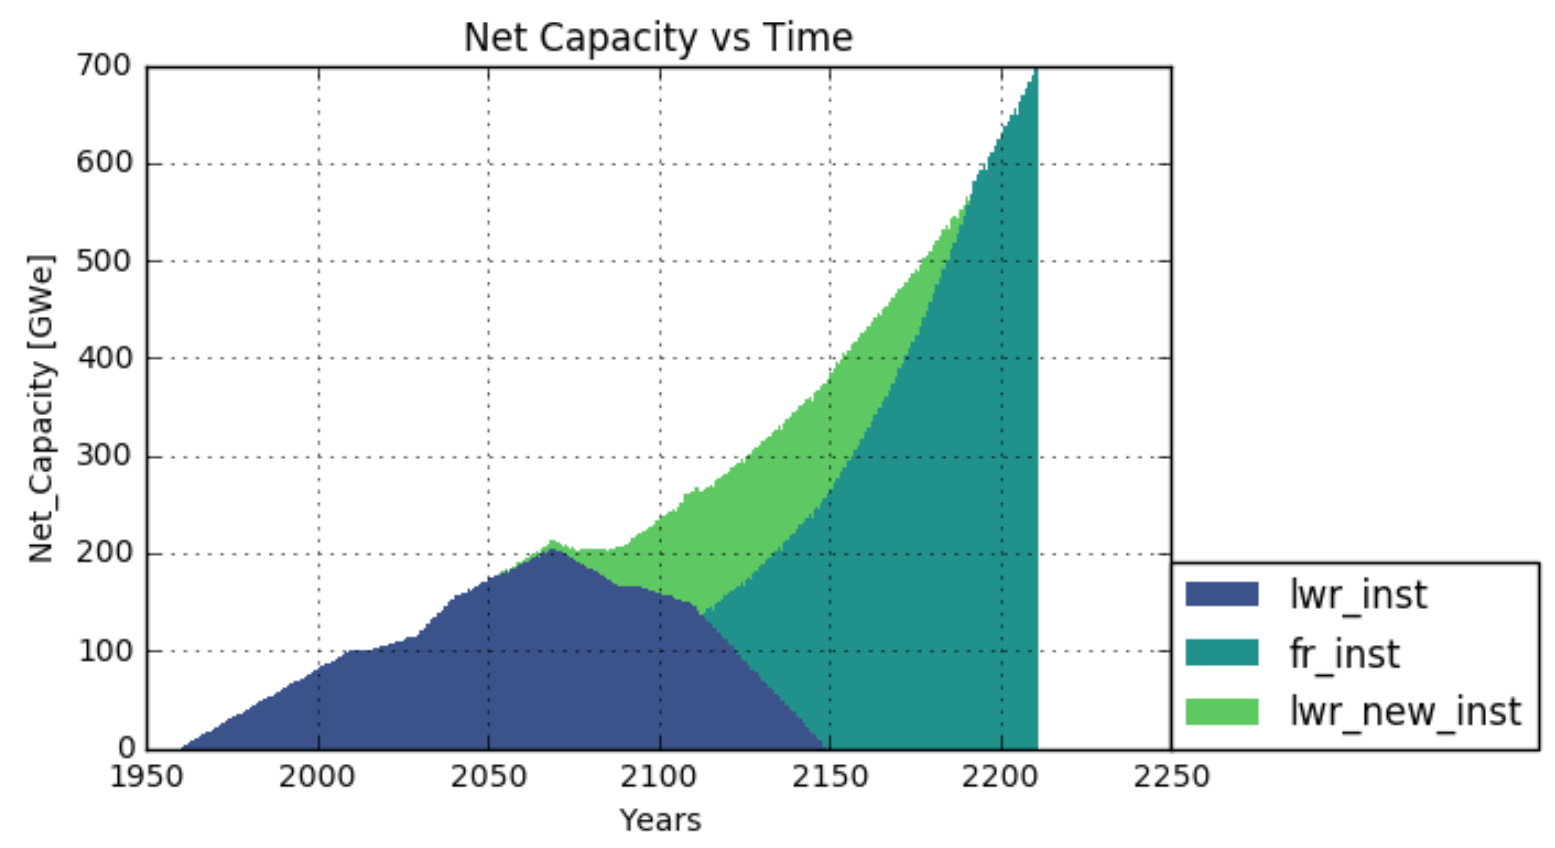
\includegraphics[width=\linewidth]{images/netcap}
\end{figure}
\end{frame}

\begin{frame}
\frametitle{Diversion Settings}
\begin{columns}
	\column[t]{4cm}
	Two Pyre prototypes:
	\begin{itemize}
		\item LWR vs SFR
	\end{itemize}
	LWR Pyre:
	\begin{itemize}
		\item Fewer diversions
		\item More material per instance
		\item Less frequent
	\end{itemize}
	SFR Pyre:
	\begin{itemize}
		\item Frequent diversion
		\item Small quantities
	\end{itemize}
	\column[t]{7cm}
	\begin{figure}
		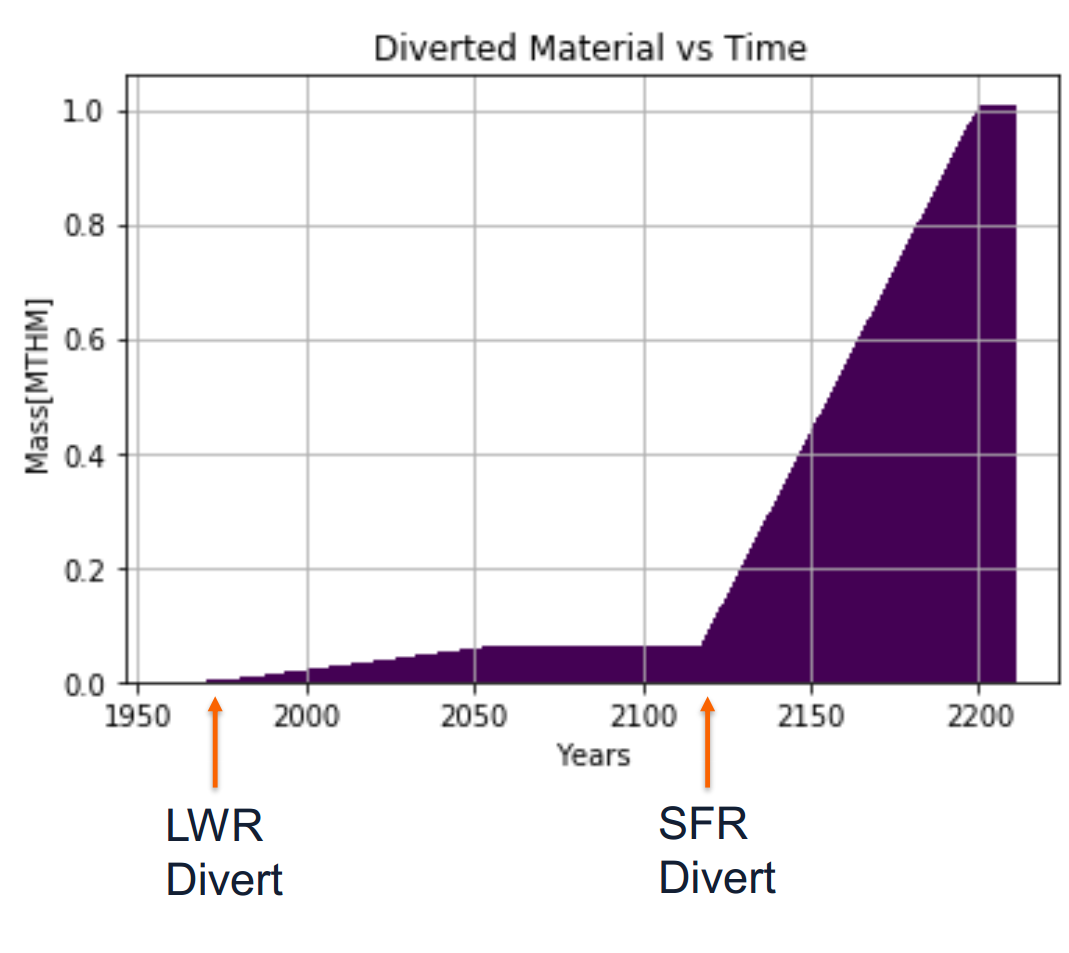
\includegraphics[width=\linewidth]{images/divertmat}
	\end{figure}
\end{columns}
\end{frame}

\begin{frame}
\frametitle{Transition Scenario - Utilization}
\begin{figure}
	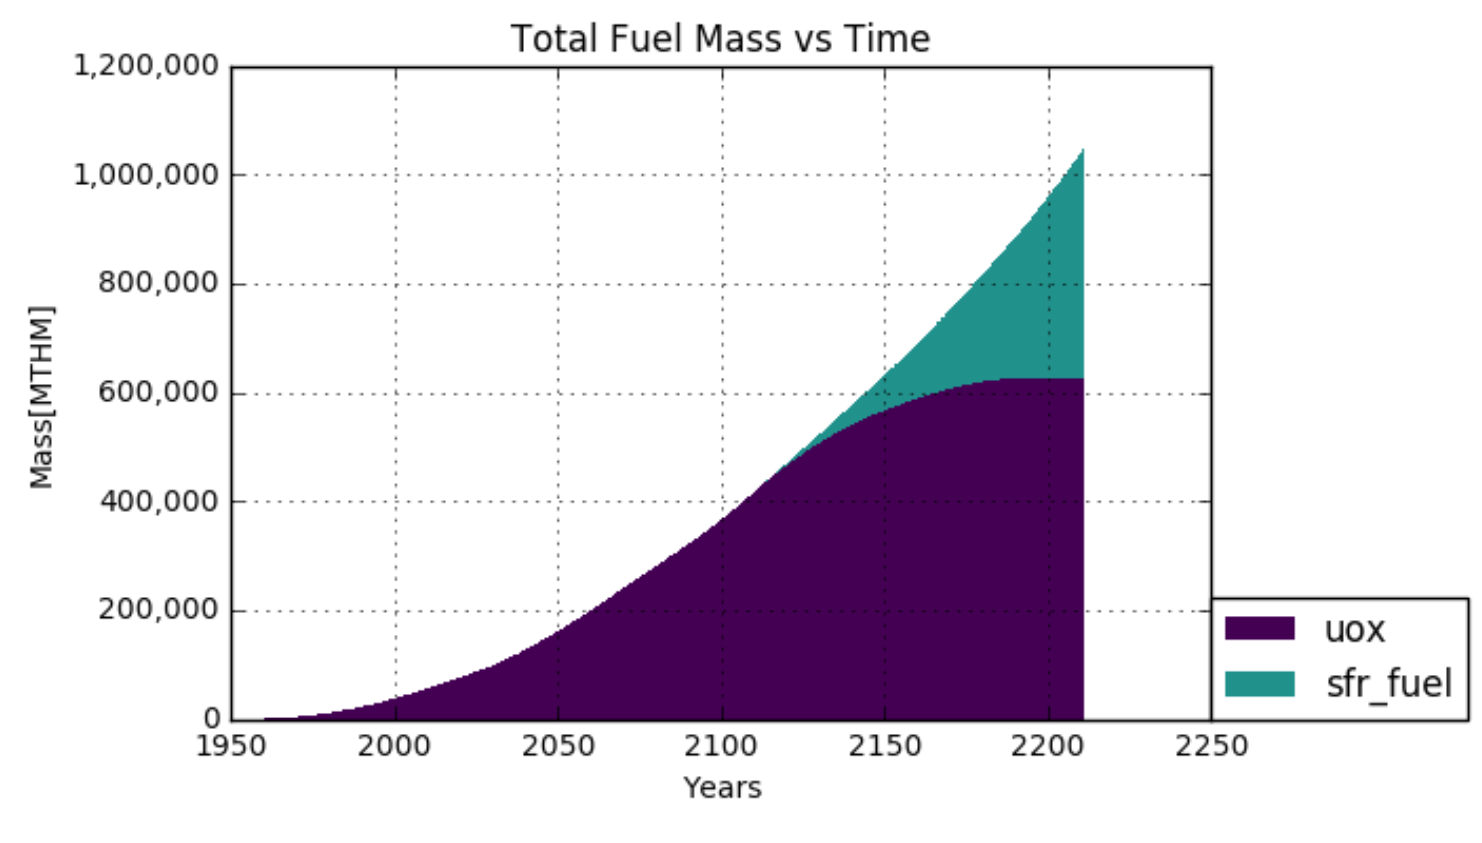
\includegraphics[width=\linewidth]{images/fuelmass}
\end{figure}
\end{frame}

\begin{frame}
\frametitle{Conclusions}
We have developed a customizable method of diverting material
from inside Cyclus facilities.
\begin{itemize}
	\item Preliminary work has been done on the detection of two
	different types of diversion: Nefarious and Operator
\end{itemize}
PyRe was demonstrated to function as both LWR and SFR
reprocessing method
\begin{itemize}
	\item Generic facility capable of modeling multiple facility layouts
\end{itemize}
\end{frame}